\chapter{The seL4 Device Driver Framework}\label{ch:sddf}
Unfortunately, many approaches to solving the issues with I/O are limited 
by the monolithic kernel design itself. This presents a strong argument to
redesign a performant yet secure I/O framework on a different architecture completely: the microkernel.
However, the microkernel design has the potential to degrade performance as it requires
significantly more context switches than its monolithic counterpart.
In order to overcome potential performance degradation in I/O systems due to this, we require a simple
framework that minimises system calls when possible for designing performant I/O systems on a microkernel architecture.
This introduces the seL4 Device Driver Framework as an excellent starting point for this project.\\

\begin{figure}[h]
    \centering
    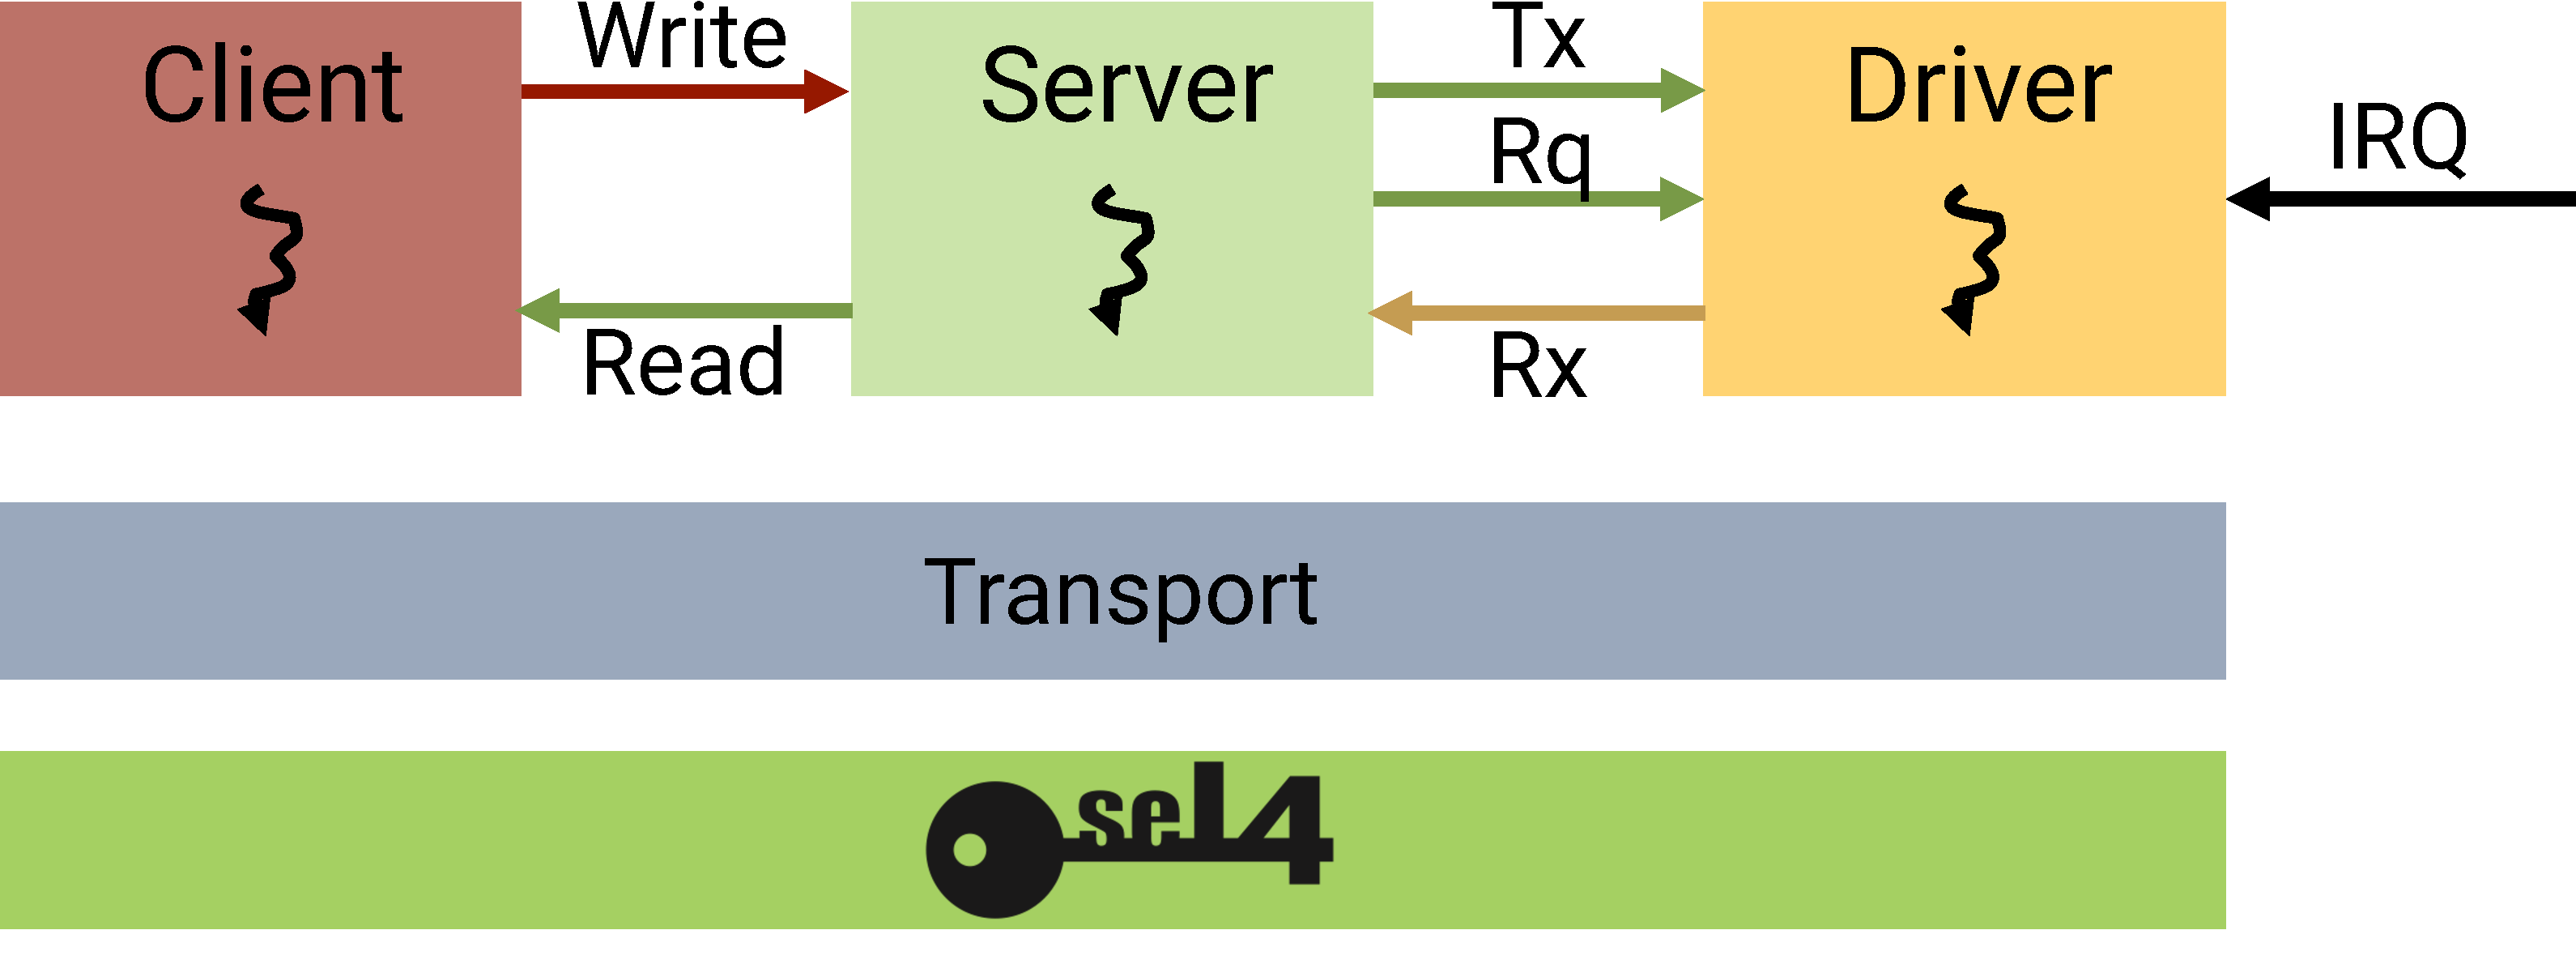
\includegraphics[width=12cm]{sddf.pdf}
    \caption{The seL4 Device Driver Framework (sDDF) \cite{Parker_22:sddf}}
    \label{f:sddf}
\end{figure}

The seL4 Device Driver Framework (sDDF) aims to rectify any performance degradation of a microkernel
design by providing interfaces and protocols to write performant yet secure user level device
drivers on seL4 \cite{Parker_22:sddf}. It currently supports a minimal networking-focused system, and is 
developed on top of the seL4 Core Platform. The sDDF prioritises a strong separation of 
concerns by componentising each task in an I/O framework such that each component has only a 
single job. For a device driver, this job is hardware abstraction. The sDDF design is based on
top of a simple transport layer that provides protocols for communication between drivers and other
components in the system.

\section{Driver Model}\label{s:driver_model}
The device driver translates a hardware specific device protocol into a hardware independent
(but OS specific) device class protocol. It is inherently event driven, as it only needs to react to
either a client request or an interrupt generated by hardware, and in this way, it maps perfectly onto
the seL4 Core Platform model. Clients make requests through shared memory and seL4 asynchronous notifications
which simplifies the device driver code to an event loop reacting to either client requests or hardware
events as shown in \autoref{l:driver_pseudo}. 

\begin{lstlisting}[tabsize=2, language=C, caption={Driver pseudo code},frame=tb, label={l:driver_pseudo}, captionpos=b]
    main() {
        init()
        while(true)
            event = Wait()
            if (event & IRQ)
                handle_irq()
            if (event & CLIENT_REQ)
                handle_request()
    }
\end{lstlisting}

\section{Transport Layer}
The sDDF transport layer consists of 3 distinct shared memory regions, data structures for data management
and access protocols. These memory regions are:
\begin{enumerate}
    \item \textbf{Metadata region}: the control registers of a device shared between the device itself and its driver. 
    This region is volatile as it is accessed directly by the device and is mapped uncached. 
    \item \textbf{Data region}: buffers containing data that's shared between the device and PDs that require access to the data.
    This region is also accessed directly by the device, but is mapped cached as we assume the device will only access it when 
    instructed. Before and after such accesses, we need to invalidate or clean buffers to ensure cache coherency.
    \item \textbf{Control region}: data structures to manage buffers in the data region. This is shared between two PDs in the system. 
\end{enumerate}

% Something about how we can just update these regions and issue notifications.
\subsection{Control region}
The control region consists of lockless, ring buffer queues. These queues are single-producer,
single-consumer (SPSC) which keeps the implementation simple.
The queues keep track of addresses in the data region as shown in \autoref{f:control}. For simplicity,
the figure only shows the control region on the transmit path between a server and driver. Each pair of 
communicating PDs in the sDDF have their own control region and share the data region. 
The sDDF uses two queues per direction, per control region. For example, as per \autoref{f:control}, the 
Transmit Used (TxU) queue stores buffer addresses which contain data ready for transmit. 
The Transmit Free (TxF) queue stores buffer addresses available for reuse. This is duplicated for the receive path.

\begin{figure}[h]
    \centering
    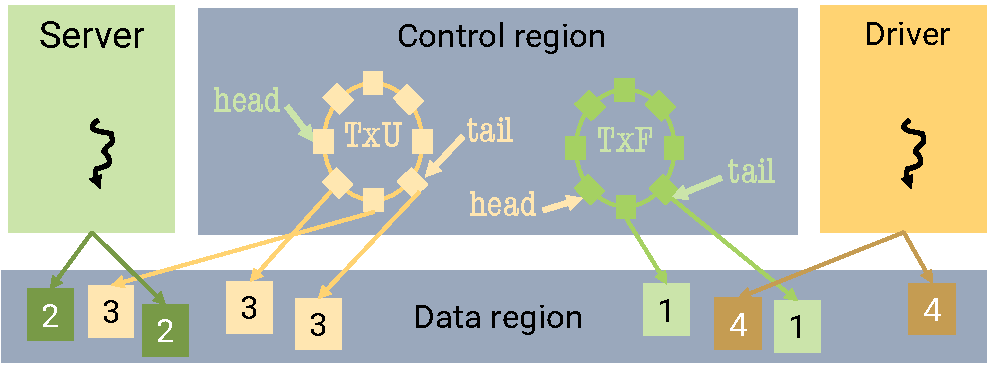
\includegraphics[width=12cm]{control_region.pdf}
    \caption{Control region between driver and server on transmit path \cite{Parker_22:sddf}}
    \label{f:control}
\end{figure}

The ring buffer queues themselves are very simple. \autoref{l:queues} shows the data structures. Each
ring buffer has a separate head and tail pointer, and entries between the tail and head point to a valid buffer
in the respective data region. Each ring buffer has exactly one producer (the server in \autoref{f:control})
and one consumer (the driver in \autoref{f:control}). The producer
only ever updates the head and the consumer only ever updates the tail.

\begin{lstlisting}[tabsize=2, language=C, caption={Ring Buffer Queues},frame=tb, label={l:queues}, captionpos=b]
    struct buffer_descr {
        void   *address;
        size_t length;
    }
    struct ring_buffer {
        uint32_t head;
        uint32_t tail;
        struct buffer_descr buffer[RING_SIZE];
    }
\end{lstlisting}

Lock free updates to these queues are possible by utilising the property that reads and writes of small
integers are atomic. We simply use a \emph{write memory barrier} before updating the head or tail pointers
as shown in \autoref{l:queues2} to ensure that no reads or writes are re-ordered by the compiler or
processor across this point. As the code ensures there is at least one unused buffer between the head and tail,
the data race is benign and the memory barrier is sufficient to ensure consistency.

\begin{minipage}{\textwidth}
\centering
\begin{lstlisting}[tabsize=2, language=C, caption={Ring Buffer Queue Management},frame=tb, 
                    label={l:queues2}, captionpos=b]
    bool full (struct ring_buffer *ring)
    {
        return (ring->head - ring->tail + 1) % RING_SIZE == 0;
    }
    bool empty (struct ring_buffer *ring)
    {
        return (ring->head - ring->tail) % RING_SIZE == 0;
    }
    void enqueue (struct buffer_descr *buffer, 
                struct ring_buffer *ring) 
    {
        assert ( !full(ring) );
        ring->buffer[ring->head % RING_SIZE] = *buffer;
        barrier();
        ring->head += 1;
    }
    struct buffer_descr* dequeue (struct ring_buffer *ring)
    {
        struct buffer_descr *buffer;
        if (empty(ring)) {
            return NULL;
        } else {
            *buffer = ring->buffer[ring->tail % RING_SIZE];
            barrier();
            ring->tail += 1;
            return *buffer;
        }
    }
\end{lstlisting}
\end{minipage}

\section{Device Sharing}\label{s:mux_design}
In order to share a device with potentially multiple client applications, the sDDF proposes a simple PD whose 
sole concern is multiplexing the hardware. This multiplexer is implemented at layer one, meaning each client application has its
own virtualised MAC address, and the multiplexer keeps a 1 to 1 mapping of MAC addresses and client CC ids. The multiplexer
can be separated into two separate components. One component handles incoming traffic (Rx Mux), and the other, outgoing traffic
(Tx Mux) as shown in \autoref{f:mux}. Control regions are used by each of these components to communicate with the component on 
either side.
In order to prevent clients from the ability to access each others' data, the shared data region must be split into
separate pools, and a simple copy component per client is responsible for copying data from one memory region to another.
\begin{enumerate}
\item \textbf{Shared Rx data region}: This data region is accessed directly by the device for writing newly received data, as well
as into the Rx Mux's address space and each of the copy components.
\item \textbf{Client Rx data regions}: This data region is mapped into a particular client's address space as well as this
client's copy component. There is a separate client Rx data region per client. The copy component copies data from the 
shared RX data region to the client's own Rx data region.
\item \textbf{Client Tx data regions}: This data region is accessed directly by the device to transmit data, but is also mapped into
the Tx Mux's address space and a particular client's address space. There is one client Tx data region per client. This
enables a zero copy interface on the transmit path.
\end{enumerate}

\begin{figure}[h]
    \centering
    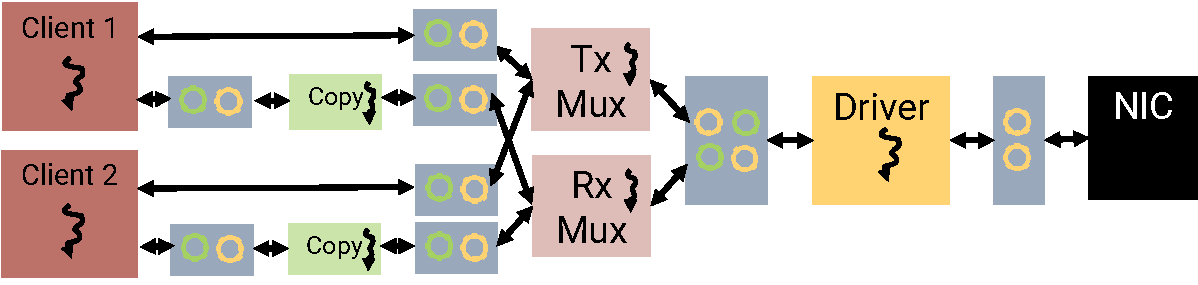
\includegraphics[width=\textwidth]{mux_design.pdf}
    \caption{Multiple client applications on the sDDF}
    \label{f:mux}
\end{figure}

A multiplexer servicing multiple components inherently requires a policy to determine the order in which it will process work.

The Rx Mux uses a FIFO policy, whereby incoming packets are passed on to the respective client, and this client is notified in the 
order in which the packets arrived. If a client's incoming queue becomes full, the multiplexer will drop any further
incoming packets for that client.

The Tx Mux could implement one of the below policies depending on the particular use case of the system:
\begin{enumerate}
\item \textbf{Round-robin}: whereby the multiplexer processes an outgoing request one at a time, alternating between clients.
\item \textbf{Priority-based}: whereby the multiplexer prioritises client requests as per their given priority, processing as many
requests as available for the highest priority client possible. 
\item \textbf{Throughput-based}: whereby the multiplexer limits the available outgoing bandwidth per client at a time.
\end{enumerate}
Rather than catering to all possible use cases and prescribing a generic policy, the sDDF instead prescribes 
keeping the policy simple and implementing one of the above policies for 
a particular use case. Should the need arise, this policy could be swapped out for another at run time. Currently,
none of these policies have been implemented.

\section{Control Flow}
Each component in the sDDF, aside from the client applications, is a single-threaded event-driven program. The
components are simply reacting to an update in either the control or metadata regions, signalled by an seL4 notification. 
To minimise the number of system calls, each component processes as many buffers as it can before signalling the next
relevant component.
The driver runs at the highest priority in the framework. This ensures timely handling of interrupts, as well
as immediate reaction to requests. In order to prevent the driver from monopolising the processor in the case
of high traffic on the receive path, we can limit the size of the receive queue in the metadata region and/or 
the size of the receive queues in the control regions.
The remaining priority ordering is as follows:

\centerline{Clients and per client copiers \(<\) Rx Mux \(<\) Tx Mux \(<\) Driver.}

This priority ordering enables components on the receive path to process as many packets as possible and
thus batch system calls. Due to the bounded size of the queues, only a limited number of packets 
can be processed in one invocation which provides flow control for lower priority components. Note that
client applications may have different priorities. In the case that client A has higher priority
than client B, then it may make sense that client B's copier has lower priority than that of client A.
However, to enable batching, clients should run at lower priority than their copy component. 
On the transmit path, components are invoked as soon as packets are 
ready to be transmitted which keeps transmit latencies low.

\section{Preliminary Evaluation}

Fine grained modularity in I/O systems, exhibited in the sDDF design, has the
potential to degrade performance because of the extra number of context switches involved.
Before embarking on the remainder of this thesis, we can already demonstrate that such a
design is feasible for simple high performance I/O systems.

\subsection{Evaluation setup}
The sDDF currently supports a minimal networking-focused system capable of echoing Ethernet packets it receives. It
runs on a single core of a Freescale i.MX 8M Mini quad applications processor with 2Gb RAM, running at 1.2 GHz with a 1Gbps NIC.
The test system comprises of the following 5 PDs:
\begin{enumerate}
\item Ethernet Driver: a minimal driver based on \ref{s:driver_model}.
\item Rx Mux: a minimal receive path multiplexer that reads the Ethernet header and compares the
destination MAC address as per \ref{s:mux_design}.
The multiplexer was developed to support one client only and does not contain any policy logic. 
\item Tx Mux: a minimal transmit path multiplexer as per \ref{s:mux_design} that supports a single
client. Similarly, it also does not contain any policy logic.
\item Copy Component: a component that copies data from the shared data region to the client's own address space. 
\item Client: an echo server. The client uses lwIP \cite{Dunkels_01} as an IP stack library to process incoming 
UDP packets and simply send them back unmodified. 
\end{enumerate}

We use ipbench \cite{Wienand_Macpherson_04} as a distributed load generator to send 1472byte sized UDP packets to test the seL4 based system. 
ipbench runs on a 4-node x86 cluster and counts the number of successful replies from the target system to measure the achieved throughput and latencies.

We compare the seL4 based system against a Linux system (version 6.1.1) on the same hardware. We use a simple user level application which 
reads and then writes all packets immediately back using sockets as described in \ref{s:sockets}. 
In order to determine the CPU utilisation of both systems, we run an idle thread at low priority to count the number of idle cycles. 

\subsection{Results}

\begin{figure}[h]
    \centering
    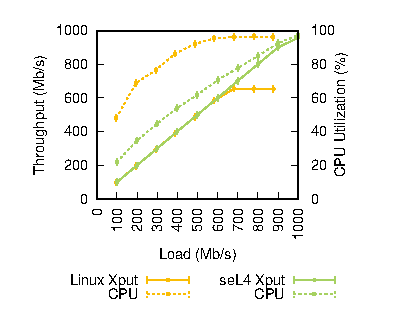
\includegraphics[width=12cm]{5comp.eps}
    \caption{Linux vs seL4 Networking Performance}
    \label{f:perf}
\end{figure}

\autoref{f:perf} compares the performance (achieved throughput and CPU utilisation over applied load) of both systems. 
We can see that the sDDF based system's throughput scales with applied load and manages to saturate the wire, while
Linux scales linearly to about 650 Mb/s and then plateaus. When comparing the CPU utilisation of both systems, we
can see that the reason behind this plateau in throughput is because Linux uses significantly more CPU cycles 
to handle a given load than the sDDF based system. Furthermore, the CPU utilisation of the sDDF system also scales 
sub-linearly with increasing load which indicates efficient batching.

\begin{figure}[h]
    \centering
    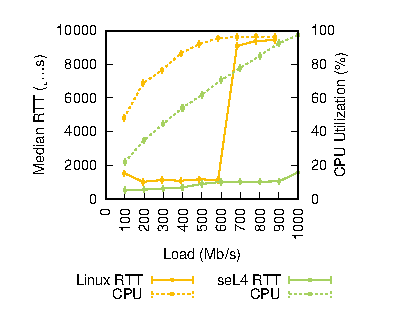
\includegraphics[width=12cm]{latency.eps}
    \caption{Linux vs seL4 Networking Latencies}
    \label{f:perf_latencies}
\end{figure}

\autoref{f:perf_latencies} compares the round trip time (RTT) latency and CPU utilisation over applied load of both systems. The latency measured
is the median result taken from a sample size of 200,000 packets. We can see that the sDDF demonstrates a much faster round trip time over Linux, 
and, unlike Linux, the round trip time does not blow up as the system becomes saturated. 

\subsection{Current Limitations}
The above results demonstrate that a simple, componentised networking system on seL4 can achieve higher throughput and lower latencies than a typical
networking system on a monolithic kernel. However, the current prototype does not currently support multiple client applications and 
is limited to single core systems. As such, the multiplexer components are very simple and do not contain any policies. Furthermore, the 
preliminary evaluation is limited as it only tests a system with symmetric traffic on the receive and transmit paths. In a real
networking system, this would not be the case. For example, a web server would have much higher throughput on the transmit path than the receive path.
Finally, the above evaluation was limited to running on a single core only which is not the typical set up for high throughput networking systems.
% TODO: Add other stuff that is currently unsupported: eg device discovery, hot plugging, extension for virtual machines although this is out
% of scope for this thesis.

\section{Thesis Problem Statement}
This thesis will extend and evaluate the current seL4 Device Driver Framework 
into a full networking system that supports multiple clients with potentially asymmetric traffic 
on a multicore system and thus demonstrate a high performance networking system on seL4.
